\chapter{Setup}
\section{Protein structure}
All simulations have been done with starting configurations adapted from previous work in the group (C36 forcefield: \textcite{pap003}, \martini{} forcefield: \textcite{sara}). These configurations contain only a FERM-kinase fragment without the FAT domain and its linker (only residues 35 to 686, PDB 2J0J \autocite{structFAK}).\\
As explained in \autoref{subsub:coarsegraining} the secondary structure of proteins have to be stabilized in \martini{} using elastic networks. This was set up by \textcite{sara} to act only between backbone beads of the same domain which are within a cut-off radius of $1\,\si{\nano\metre}$. Therefore, the interface between FERM domain and kinase is not affected and the linker is still flexible. The force constant is 830 $\si{\kilo\joule\mole^{-1}\nano\meter^{-2}}$. 
\section{Setup 1 - FAK in solution}
\label{setup:setup1}
Setup 1 refers to a \martini{} simulation of a single FAK molecule in waterbox. NaCl ions were added to neutralize the charge (see \autoref{setup:setup1_pic}).\\
After a short equilibration the system was simulated for $20\,\si{\micro\second}$ at a temperature of $300\,\si{\kelvin}$. We used the default parameters of the \martini{} forcefield as input parameters.
%
%
%
\begin{figure}[h]
	\centering
	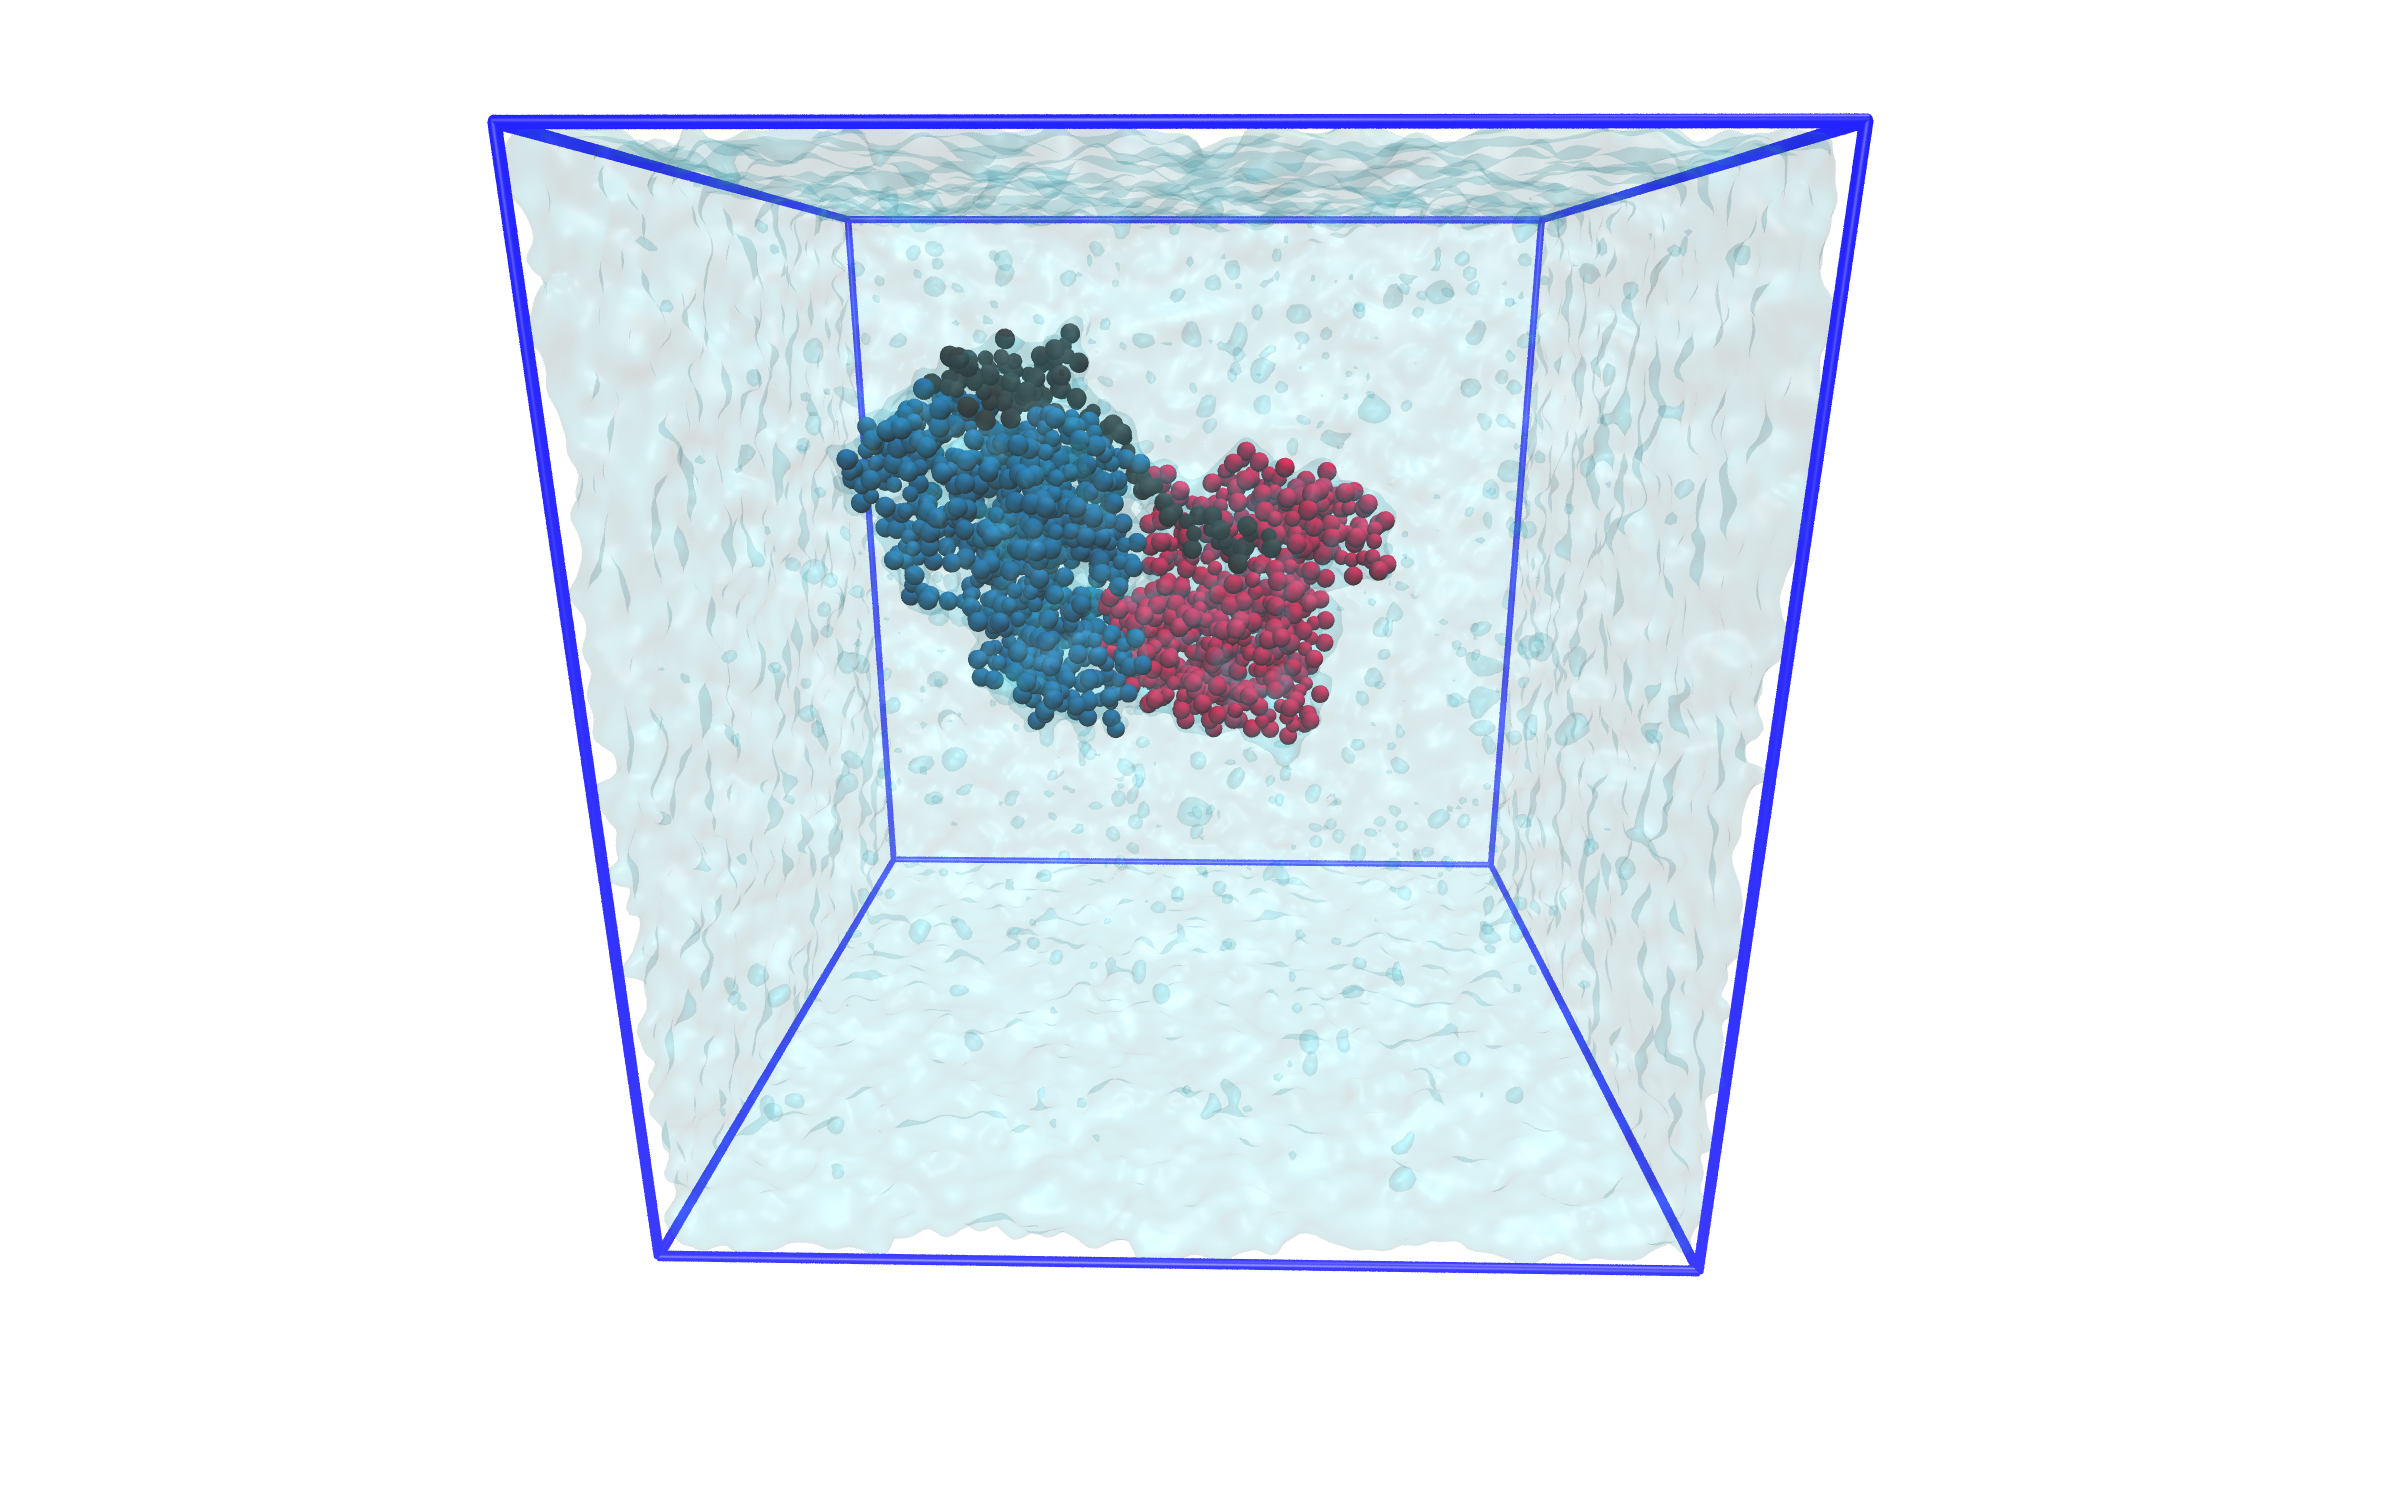
\includegraphics[height=6cm]{figures/setup/setup_free}
	\nicecaption{Setup 1 - FAK in solution}{The \martini{} structure of FAK (FERM blue, kinase red and linker black, 1486 beads) was put in a waterbox (ca. 50000 solvent beads) with ions (23 sodium beads and 20 chlorine beads). The box dimensions are $18.8\,\si{\nano\metre}$ x $18.8\,\si{\nano\metre}$ x $18.8\,\si{\nano\metre}$.}
	\label{setup:setup1_pic}
\end{figure}
%
%
%
\section{Setup 2 - Free energy of basic patch}
\label{setup:setup2}
For this setup only a part of F2 (residues 107 to 219, referred as F2 lobe in the following) was used. The lobe contains the basic patch and has a net charge of -5. Therefore no additional ions were needed.\\
We placed the lobe as a \charmm{} structure above a single \pip{} embedded into a phosphatidylethanolamine (\pope{}) membrane (see \autoref{setup:setup2_pic}). After a short equilibration, the F2 lobe was pulled slowly away from the membrane using a distance pull between the COM of the lobe and the COM of \pip{}. From this simulation, we retrieved starting conformations for the umbrella window. The number of umbrella windows was chosen accordingly to the sampling (between 90 and 120 windows). Each window was shortly equilibrated and afterwards simulated for $6\,\si{\nano\second}$.  From the trajectories of the umbrella windows the free energy profile was calculated using \gromacs{} WHAM implementation \autocite{gromacsWHAM}. The pulling and umbrella sampling was done five times to estimate the statistical error.\\
The starting configurations was transferred to a \martini{} structure (with both, standard water model and PW) with provided transformation tools \autocite{backward.py}. Afterwards the elastic network was applied. Analogously to the simulation in \charmm{}, we retrieved starting configurations for the umbrella windows and simulated them for five independent copies. The simulation time for one umbrella window was increased to $10\,\si{\nano\second}$.\\
The presented results are based on a total simulation time of $3.88\,\si{\micro\second}$ for C36, $6.33\,\si{\micro\second}$ for \martini{}, $5.64\,\si{\micro\second}$ for \martini{} with PW. The temperature in the simulations was kept at $300\,\si{\kelvin}$. For all three force fields the default parameters were used.
% C36: 1=180, 4.2=135, 5=102, 5.2=102, 6=127, Mart: 1=134, 2=126, 3=130, 4=113, 5=130, MartPol: alle=113
%
%
%
\begin{figure}[h]
	\centering
	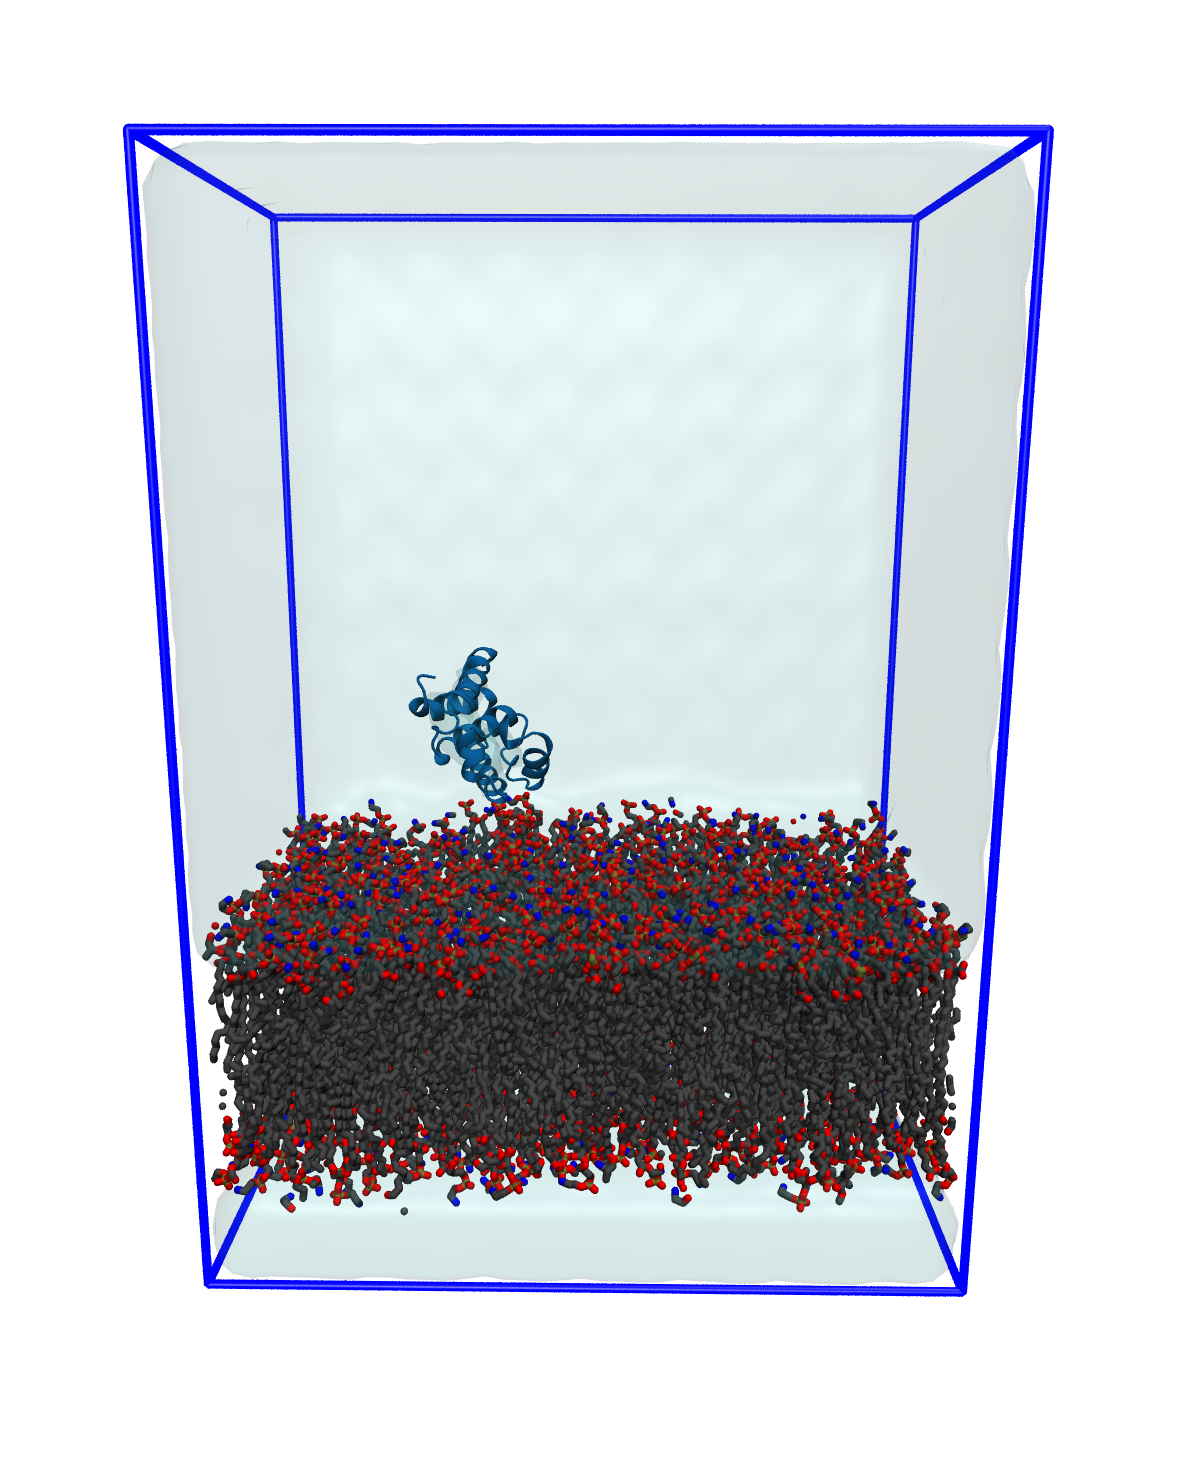
\includegraphics[height=6cm]{figures/setup/setup_umbrella}
	\nicecaption{Setup 2 - Free energy of basic patch}{The \charmm{} structure of the lobe (1936 atoms) above one \pip{} (143 atoms) embedded in a \pope{} membrane (509 lipids, ca. 63600 atoms). The box was filled up with ca. 63000 water molecules. The corresponding \martini{} structure contains 269 beads for the lobe, 6125 beads for the membrane and ca. 16200 solvent beads/PW molecules. The box dimensions are $14.0\,\si{\nano\metre}$ x $9.0\,\si{\nano\metre}$ x $20.0\,\si{\nano\metre}$.}
	\label{setup:setup2_pic}
\end{figure}
%
%
%
\section{Setup 3 - FAK on a \pip{} membrane}
\label{setup:setup3}
Setup 3 is a \martini{} simulation adopted from \textcite{sara}. It contains a single FAK molecule which was placed on a phosphatidylcholine (\popc{}) and \pip{} membrane (\pip{} concentration $15\%$). NaCl were added to neutralize the system (see \autoref{setup:setup3_pic}). In contrast to \textcite{sara}, we applied the stabilizing force explained in \autoref{motivation} to the protein.\\
Five independent copies were simulated for $10\,\si{\micro\second}$ each. The temperature was kept at $300\si{\kelvin}$ and the default parameters of \martini{} were used.
%
%
%
\begin{figure}[h]
	\centering
	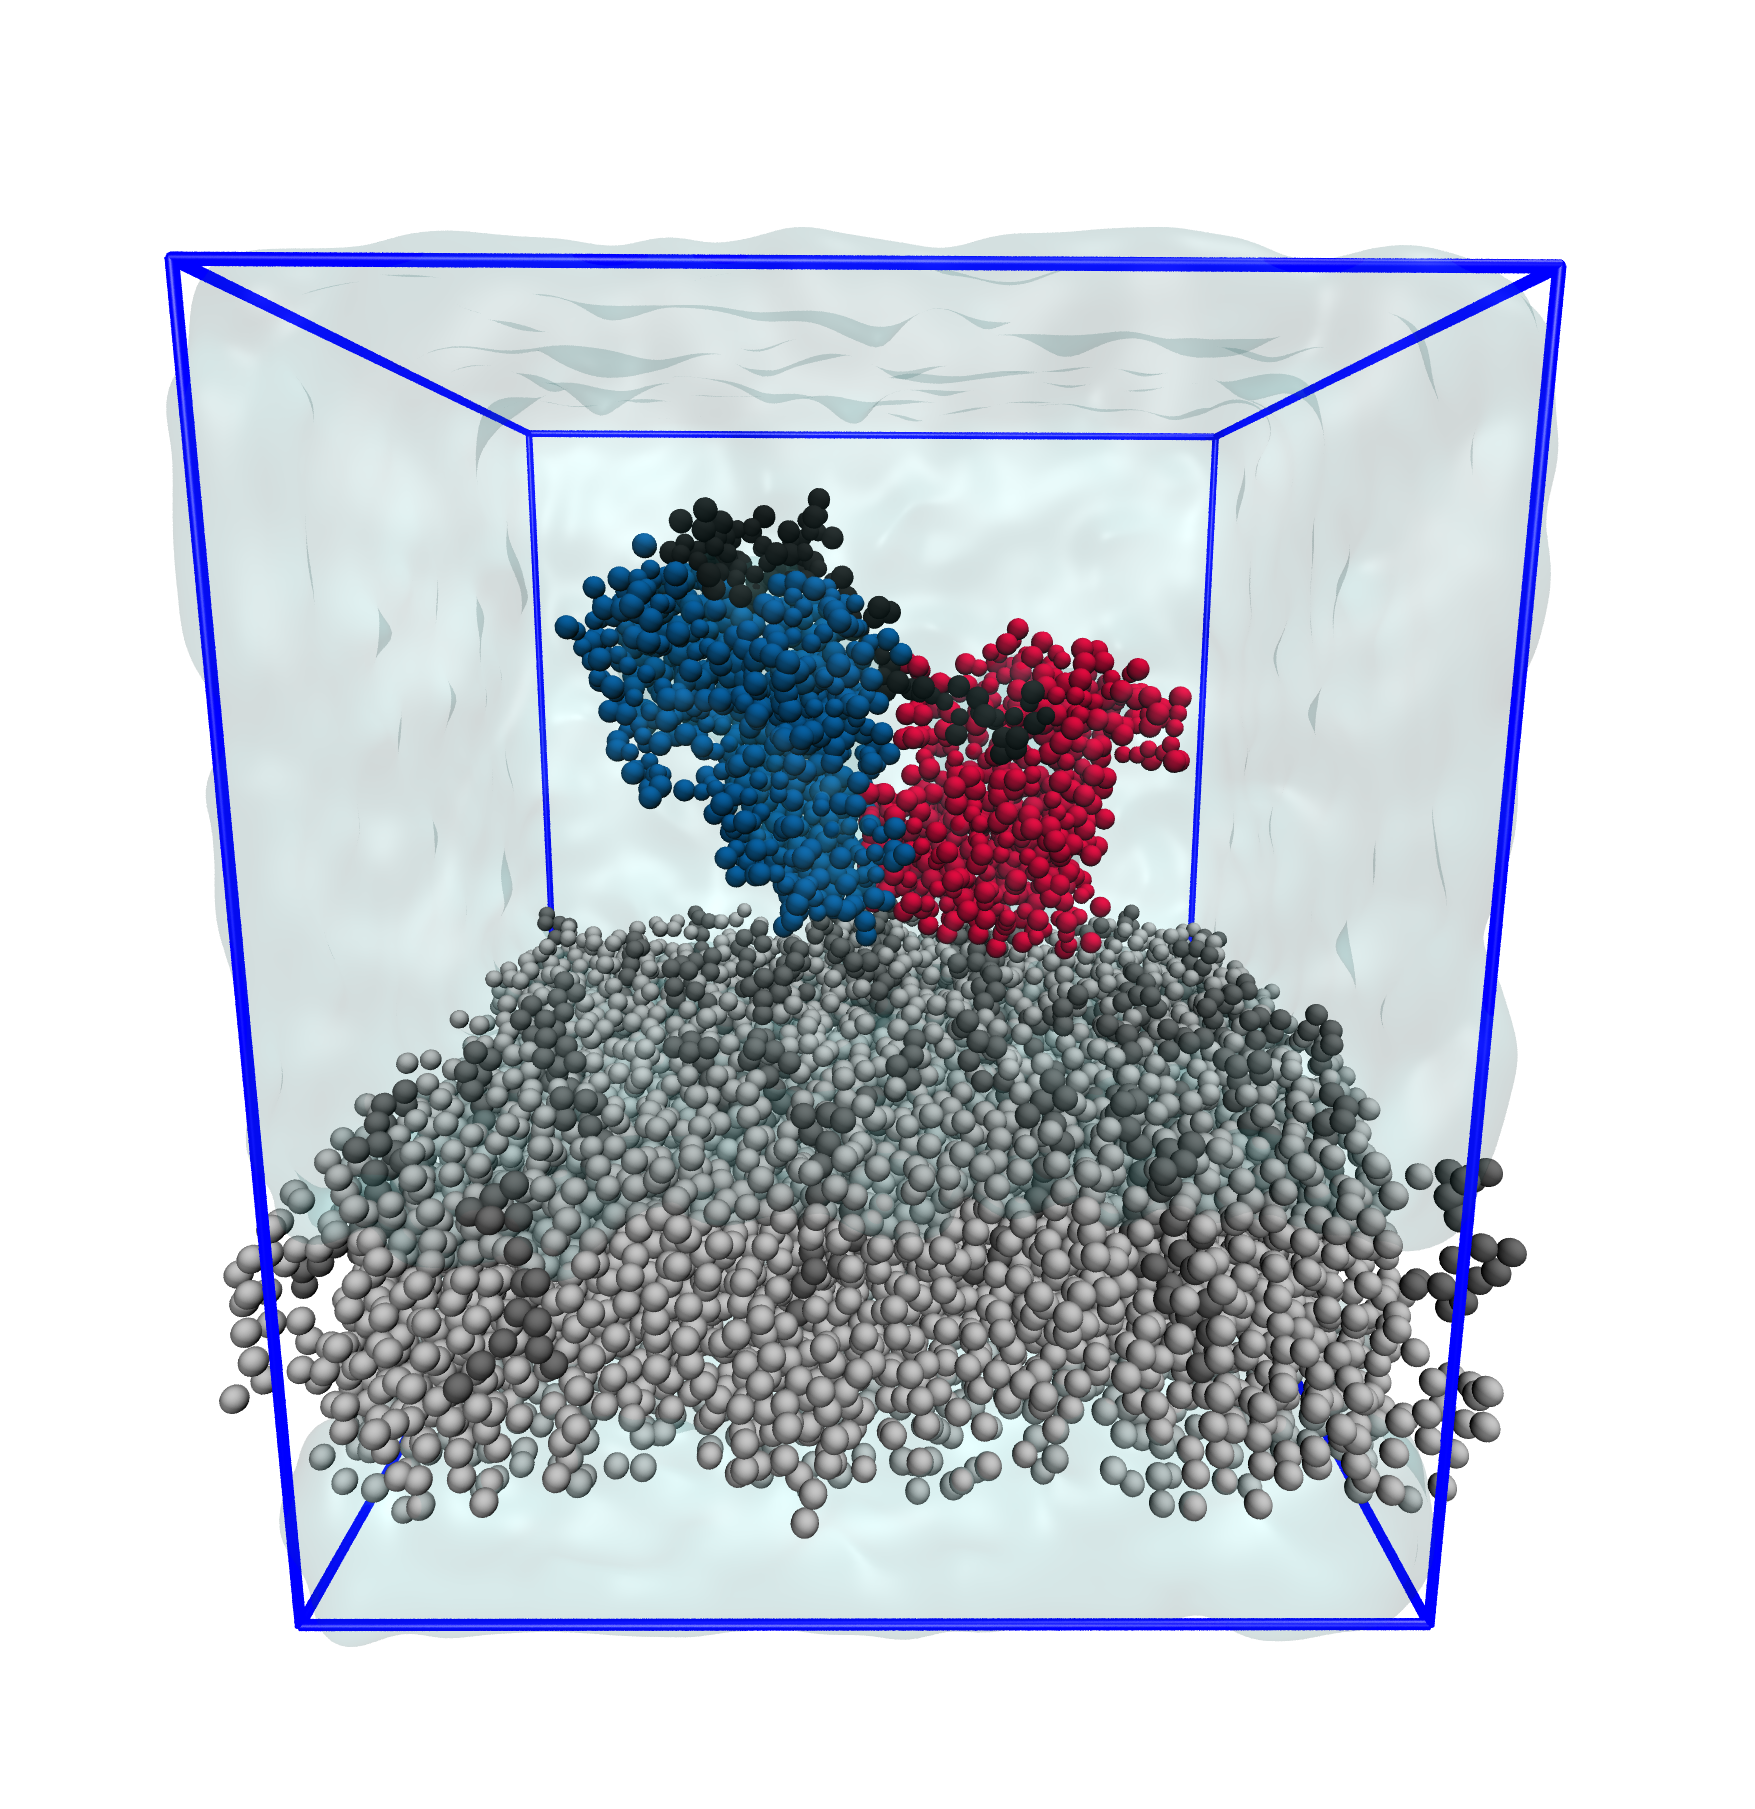
\includegraphics[height=6cm]{figures/setup/setup_gen}
	\nicecaption{Setup 3 - FAK on a \pip{} membrane}{The setup involves one FAK molecule (FERM blue, kinase red and linker black, 1486 beads) on top of a \pip{} containing membrane (XXX \pope{} lipids, XXX \pip{} lipids, XXX beads). The surrounding solution consists of XXX solvent beads and XXX ions. The box dimensions are XXX.}
	\label{setup:setup3_pic}
\end{figure}
%
%
%
\section{Setup 4 - FAK cluster}
From each copy in setup 3, we cut out five frames. All these 25 frames were arranged on a {5x5} grid (\autoref{setup:setup4_pic}). Each of the 25 proteins was stabilized with the external force independently. After a short equilibration the system was simulated for $9\,\si{\micro\second}$. We set up 25 different copies, regarding to the arrangement of the frames, resulting in a total simulation time of $45\,\si{\micro\second}$. The temperature was kept at $300\,\si{\kelvin}$ and the default parameters of \martini{} were used.
%
%
%
\begin{figure}[h]
	\centering
	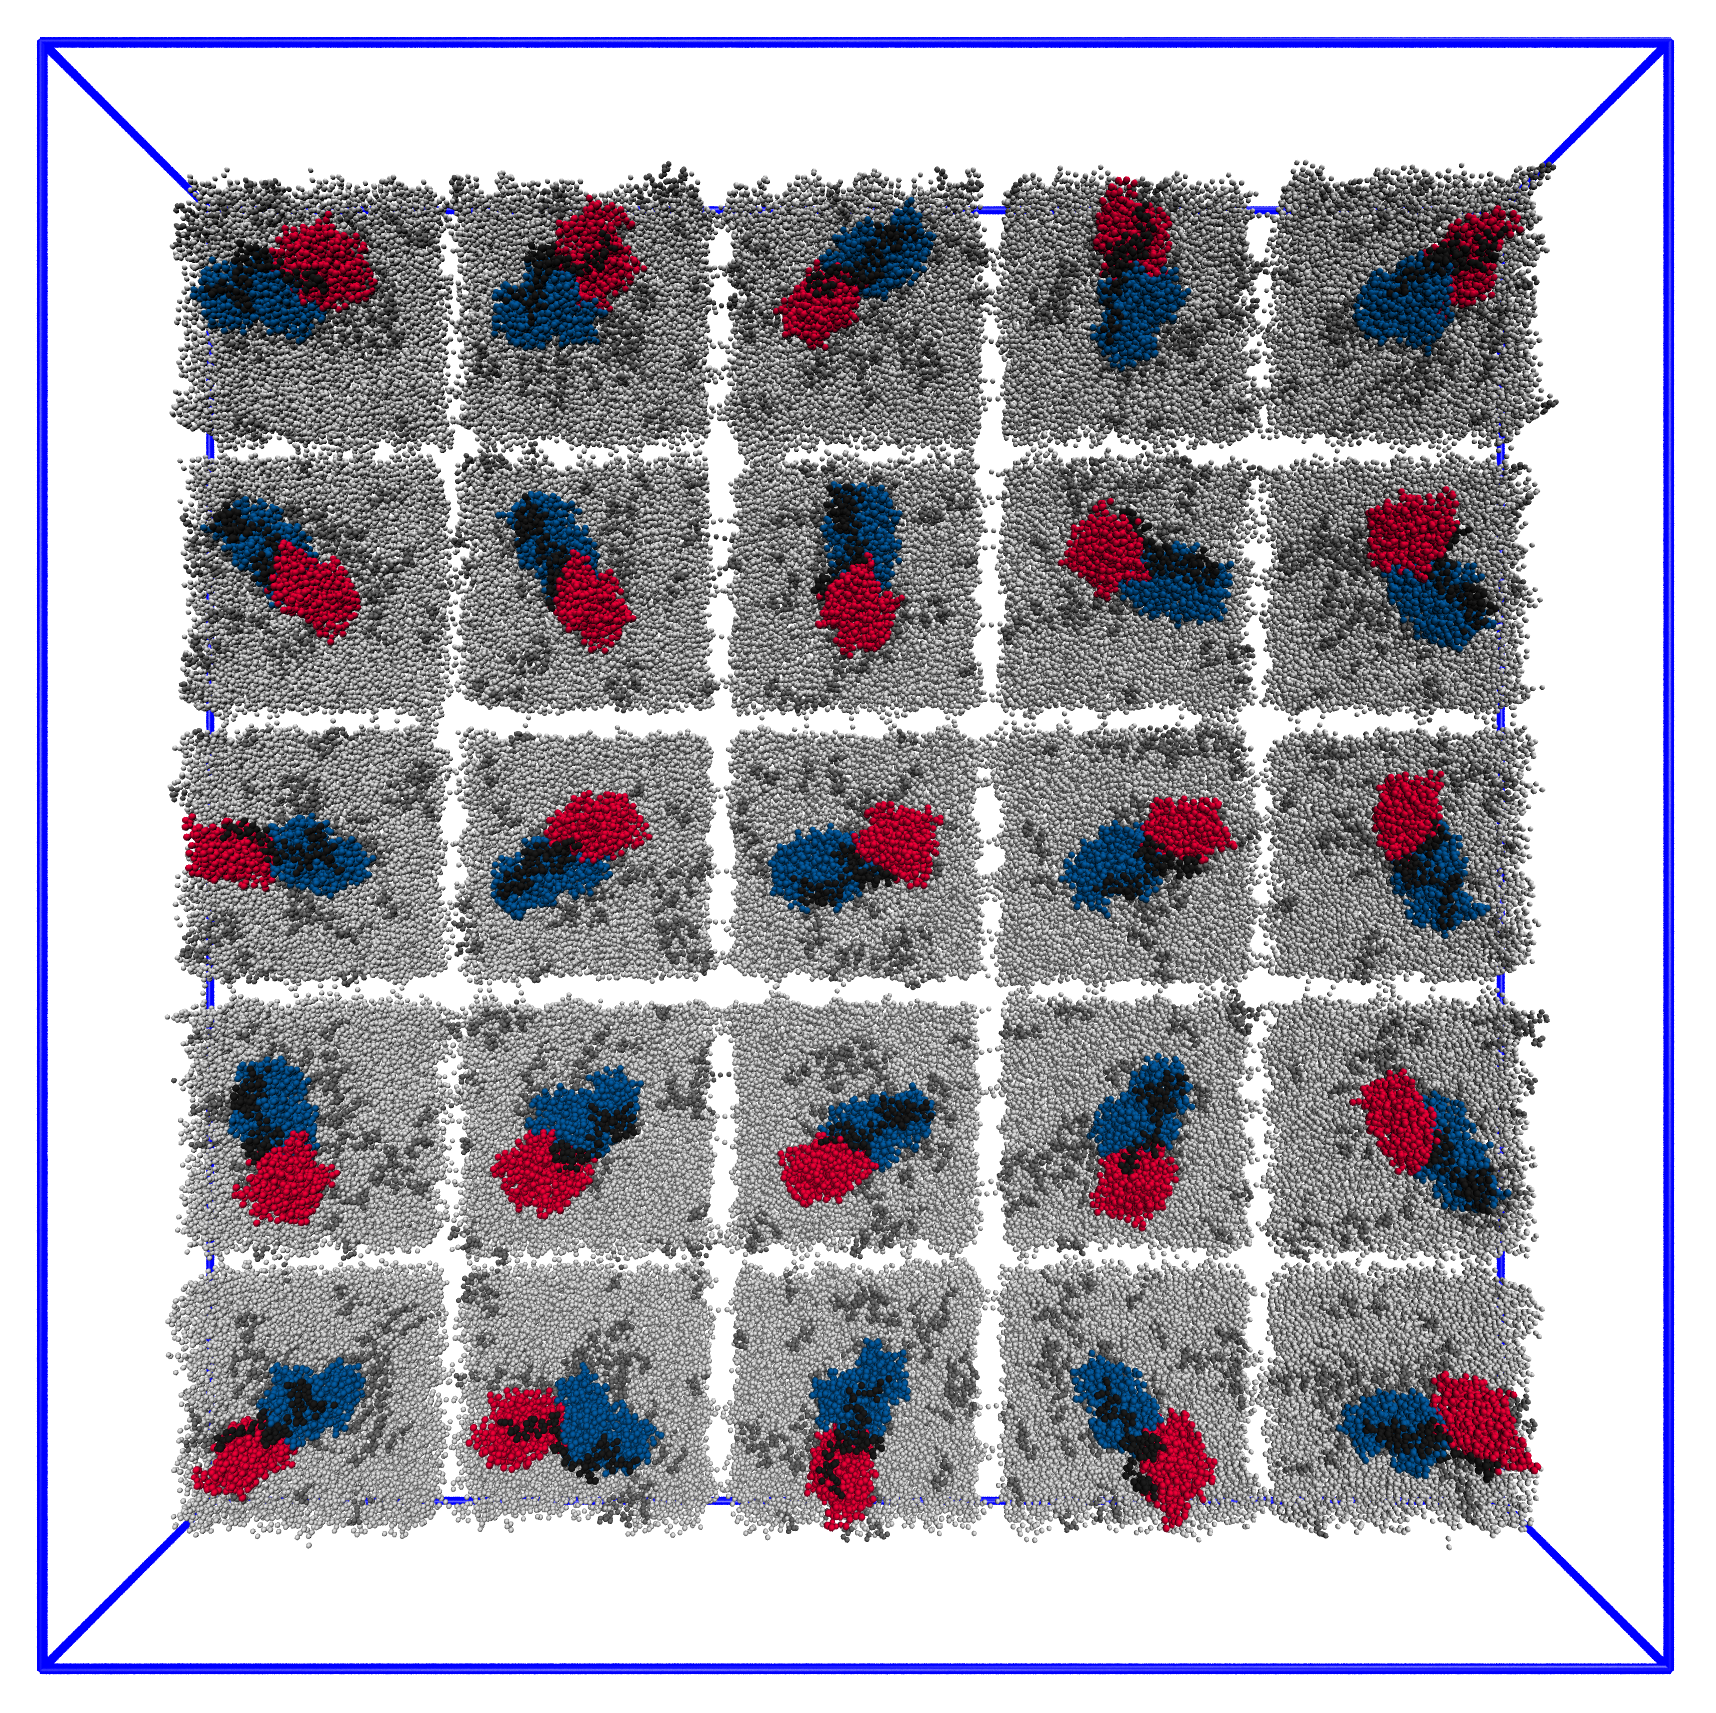
\includegraphics[height=6cm]{figures/setup/setup_cluster}
	\nicecaption{Setup 4 - FAK cluster}{The setup is a combination of 25 frames from \autoref{setup:setup3}. There are XXX beads in total, the box dimensions are XXX. The spaces between the frames were needed during setup but disappears during the equilibration.}
	\label{setup:setup4_pic}
\end{figure}
%
%
%